\documentclass[aspectratio=169]{beamer}
\mode<presentation>{
  \usetheme{default}
  \usecolortheme{dove}
}
\defbeamertemplate*{footline}{my footline}
{
	\ifnum \insertpagenumber=1
		\leavevmode%
		
\includegraphics[width=\paperwidth]{MPIM_Titelseite_unten.pdf}%NEW
		\vskip-10pt%NEW
		\hbox{%
			\pgfsetfillopacity{0}\begin{beamercolorbox}[wd=1\paperwidth,ht=2.25ex,dp=1ex,center]{title in head/foot}%
				\usebeamerfont{title in head/foot}\pgfsetfillopacity{1}%\insertframenumber{} / \inserttotalframenumber\hspace*{2ex}
			\end{beamercolorbox}%
		}%
		\vskip0pt%
	\else
		\leavevmode%
		%
\includegraphics[width=\paperwidth]{MPIM_IMPRS_Folgeseite_unten.pdf}
		
\includegraphics[width=\paperwidth]{MPIM_Titelseite_unten.pdf}		
		\vskip-10pt
		\hbox{%
			\pgfsetfillopacity{0}\begin{beamercolorbox}[wd=1\paperwidth,ht=2.25ex,dp=1ex,center]{title in head/foot}%
				\usebeamerfont{title in head/foot}\pgfsetfillopacity{1}\insertframenumber{} / \inserttotalframenumber\hspace*{2ex}
			\end{beamercolorbox}%
		}%
		\vskip0pt%
	\fi
}

%\usepackage[colorlinks=true, urlcolor=blue, linkcolor=blue,citecolor=blue]{hyperref}
%\usepackage[german]{babel}
\usepackage{float}
%\usepackage[numbers]{natbib}
\usepackage[authoryear]{natbib}
\definecolor{links}{HTML}{2A1B81}
\hypersetup{colorlinks,linkcolor=links,urlcolor=links}
\usepackage{appendixnumberbeamer}

%\let\oldcite=\cite                                                              
%\renewcommand{\cite}[1]{\textcolor[rgb]{.7,.7,.7}{\oldcite{#1}}}

\usepackage{graphicx}
\graphicspath{{/home/mpim/m300524/MSc_Thesis/gfx/}}

%\newcommand{\member}{m105_1994_2001}
%\newcommand{\member}{m178_1985_1992} % zweitbesten
\newcommand{\member}{m182_1988_1995} %funktioniert am besten

\renewcommand\refname{References and Notes}


\makeatletter
\setbeamertemplate{footline}[my footline]





\title{\vspace{1cm} \\ The impact of biology on decadal decreasing trends of carbon sink in the Southern Ocean}

\subtitle{ \vspace{1cm} Aaron Spring,$^{1}$ Hongmei Li,$^{1}$ Tatiana Ilyina$^{1}$
\\ \normalsize{$^{1}$Max Planck Institute for Meteorology, Bundesstra{\ss}e 53, 20146 Hamburg, Germany}
}



\begin{document}
\begin{frame}[noframenumbering]
	\titlepage
\end{frame}

\begin{frame}{Observations \citep{landschuetzer2015} show anomalous outgassing decadal trend in the Southern Ocean Carbon Sink in the 1990s.}
	\begin{figure}[h]
	\centering
	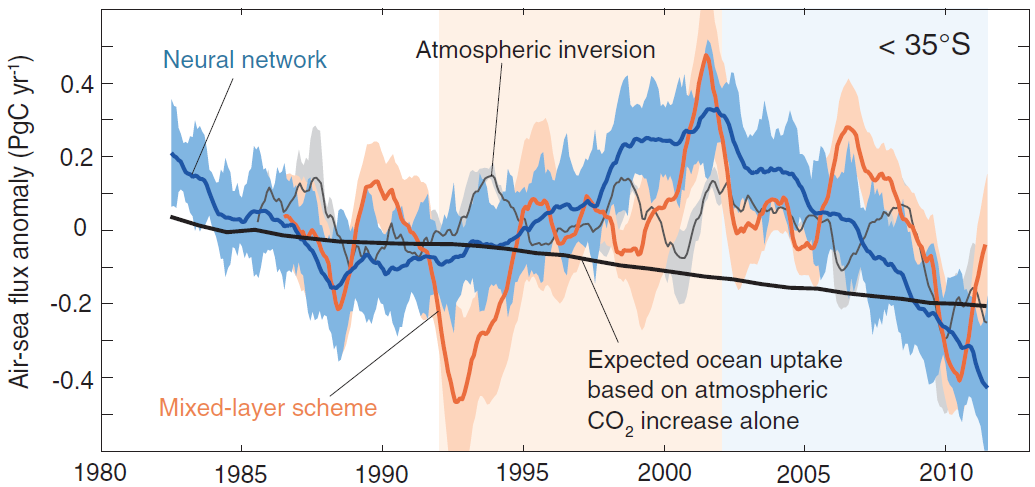
\includegraphics[scale=.3]{landschuetzer_fig1.png} % from gfx folder
	%\caption{Southern Ocean CO$_2$flux where negative values indicate ocean uptake (top) and primary production (bottom): ensemble median (left) as forced signal and ensemble standard deviation (right) as internal variability}
	\label{fig:SOCS_ensmean_ensstd}
	\end{figure}
	
\end{frame}
	
	
\begin{frame}{Decadal trends of internal variability were not yet explored in coupled earth system models. We use initially perturbed 100-member ensemble simulation to assess the variability of the Southern Ocean carbon sink and its underlying processes.}
%I identify similar decadal trends in the MPI-ESM LE.	

	\begin{figure}
		\centering
		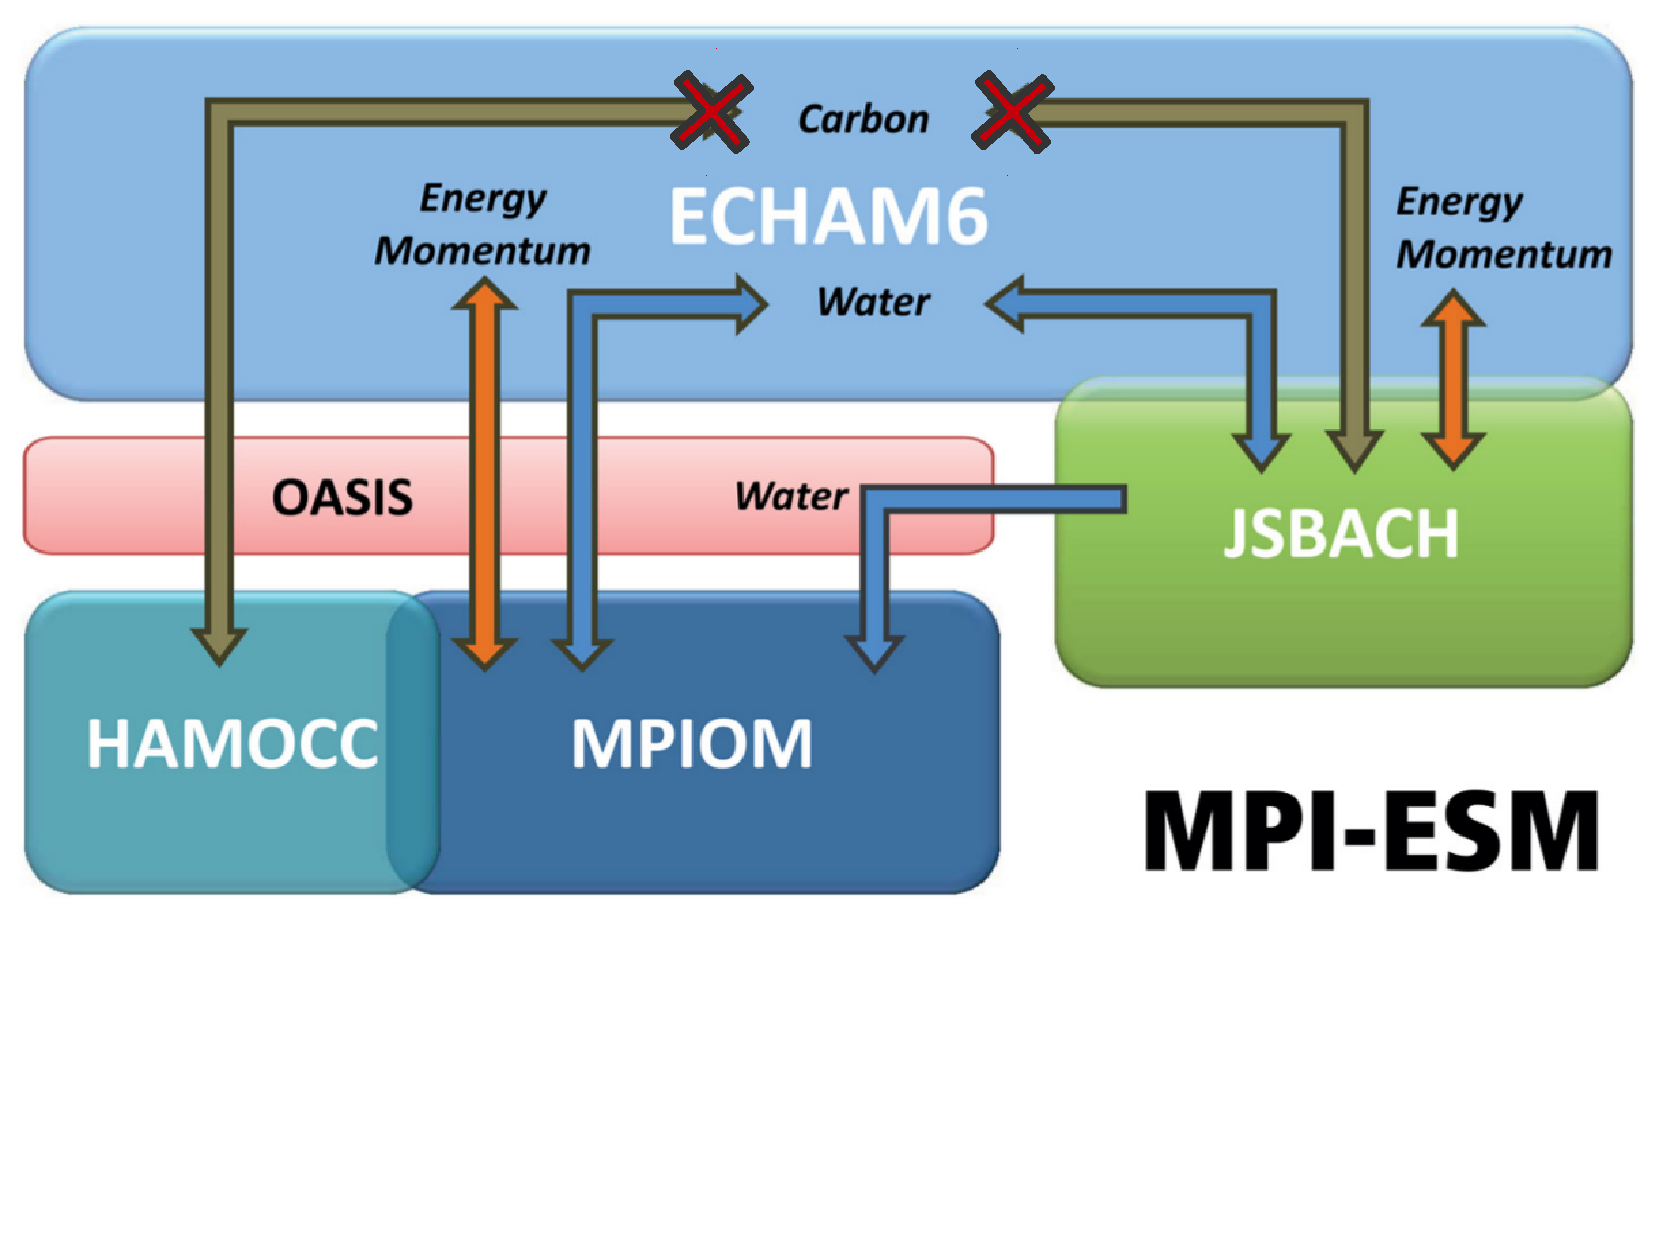
\includegraphics[scale=.3,trim=0cm 2cm 0cm 0cm,clip]{MPIESM.pdf}
	\end{figure}
\end{frame}



\begin{frame}{We find positive decadal trends in the Southern Ocean carbon sink similar to observations in the 1990s \citep{landschuetzer2015}.} 
	
	\begin{figure}
		\centering
		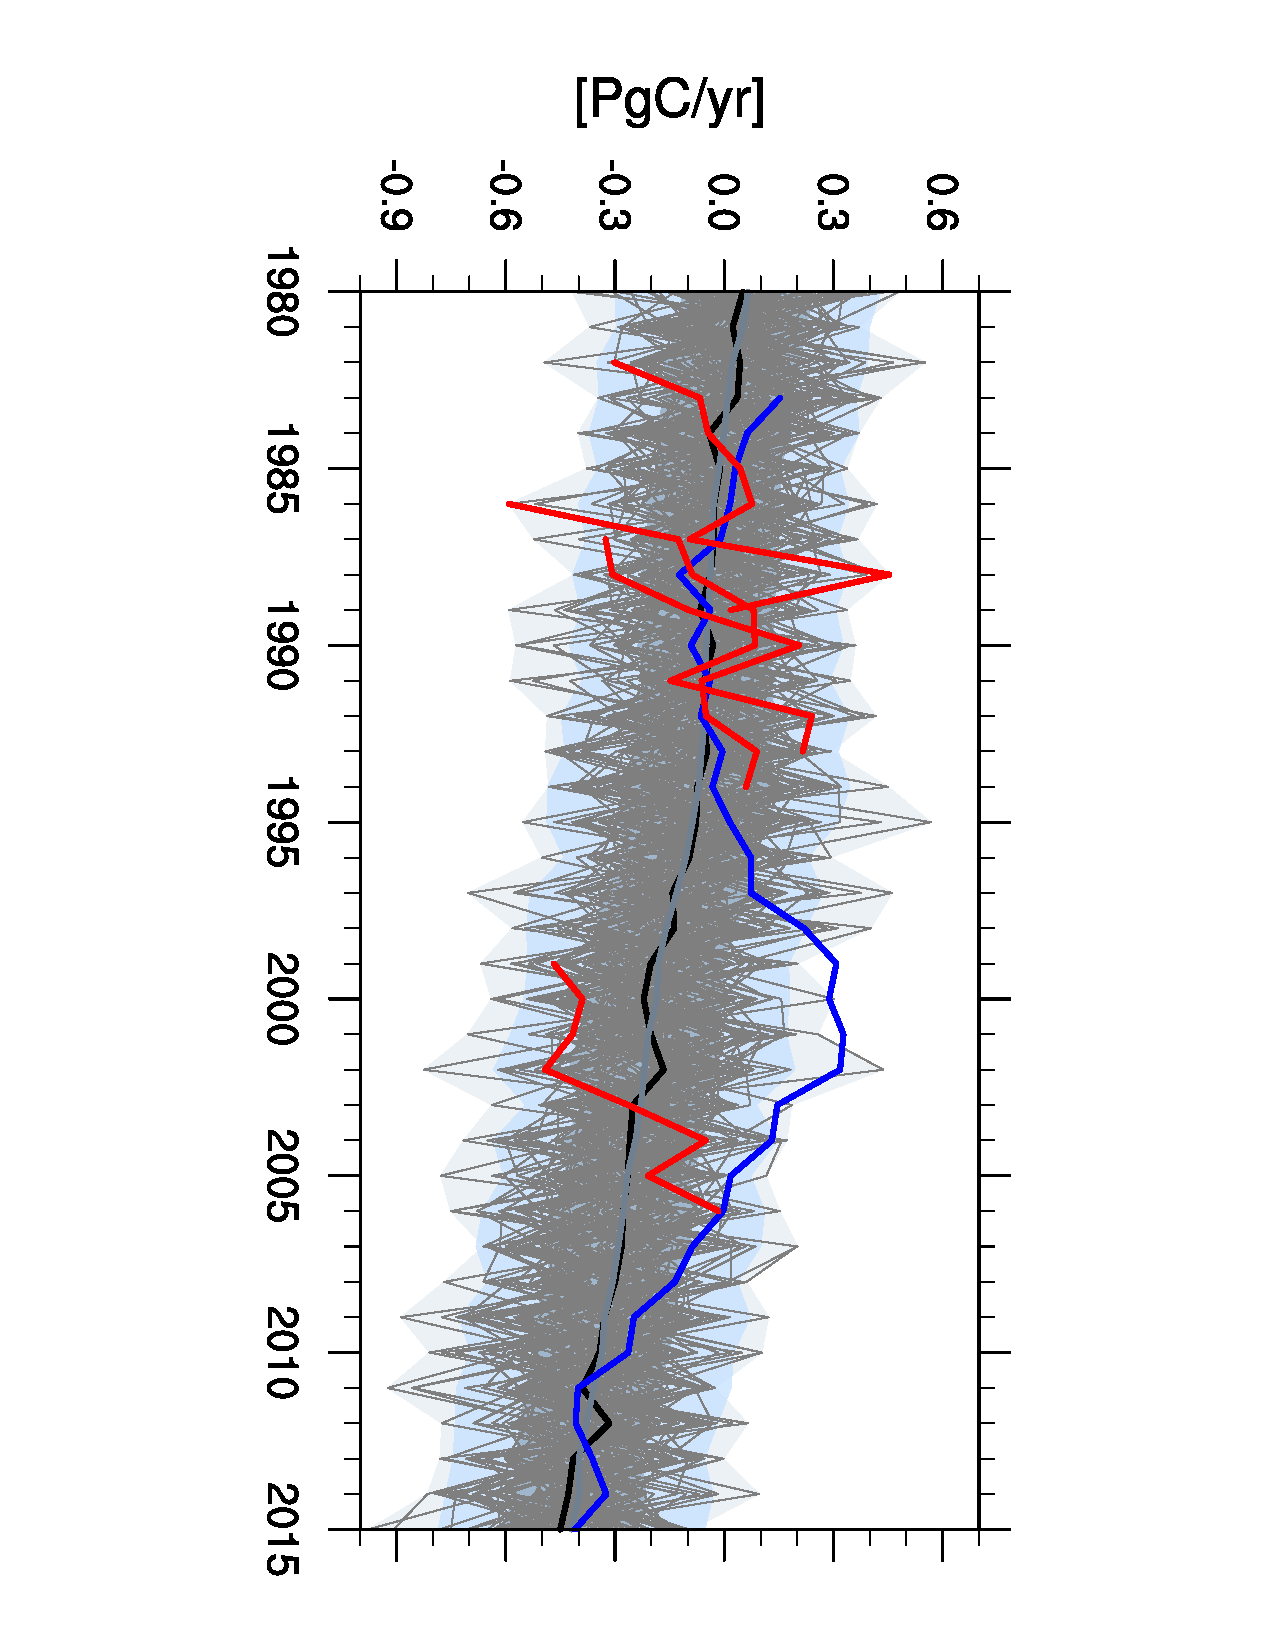
\includegraphics[scale=.45,angle=90,trim=3cm 0cm 4cm 0cm,clip]{co2flux_SO_timeseries_ym_mar-feb_35S_1980_2015_trend_8.pdf}
	\end{figure}
\end{frame}	
	
%not nessessarily needed	
\begin{frame}{Internal Variability of CO$_2$flux and primary production show similar patterns, have highest values at 45-60$^\circ$S south and appear in same locations.}  
	
	\begin{figure}
		\centering
		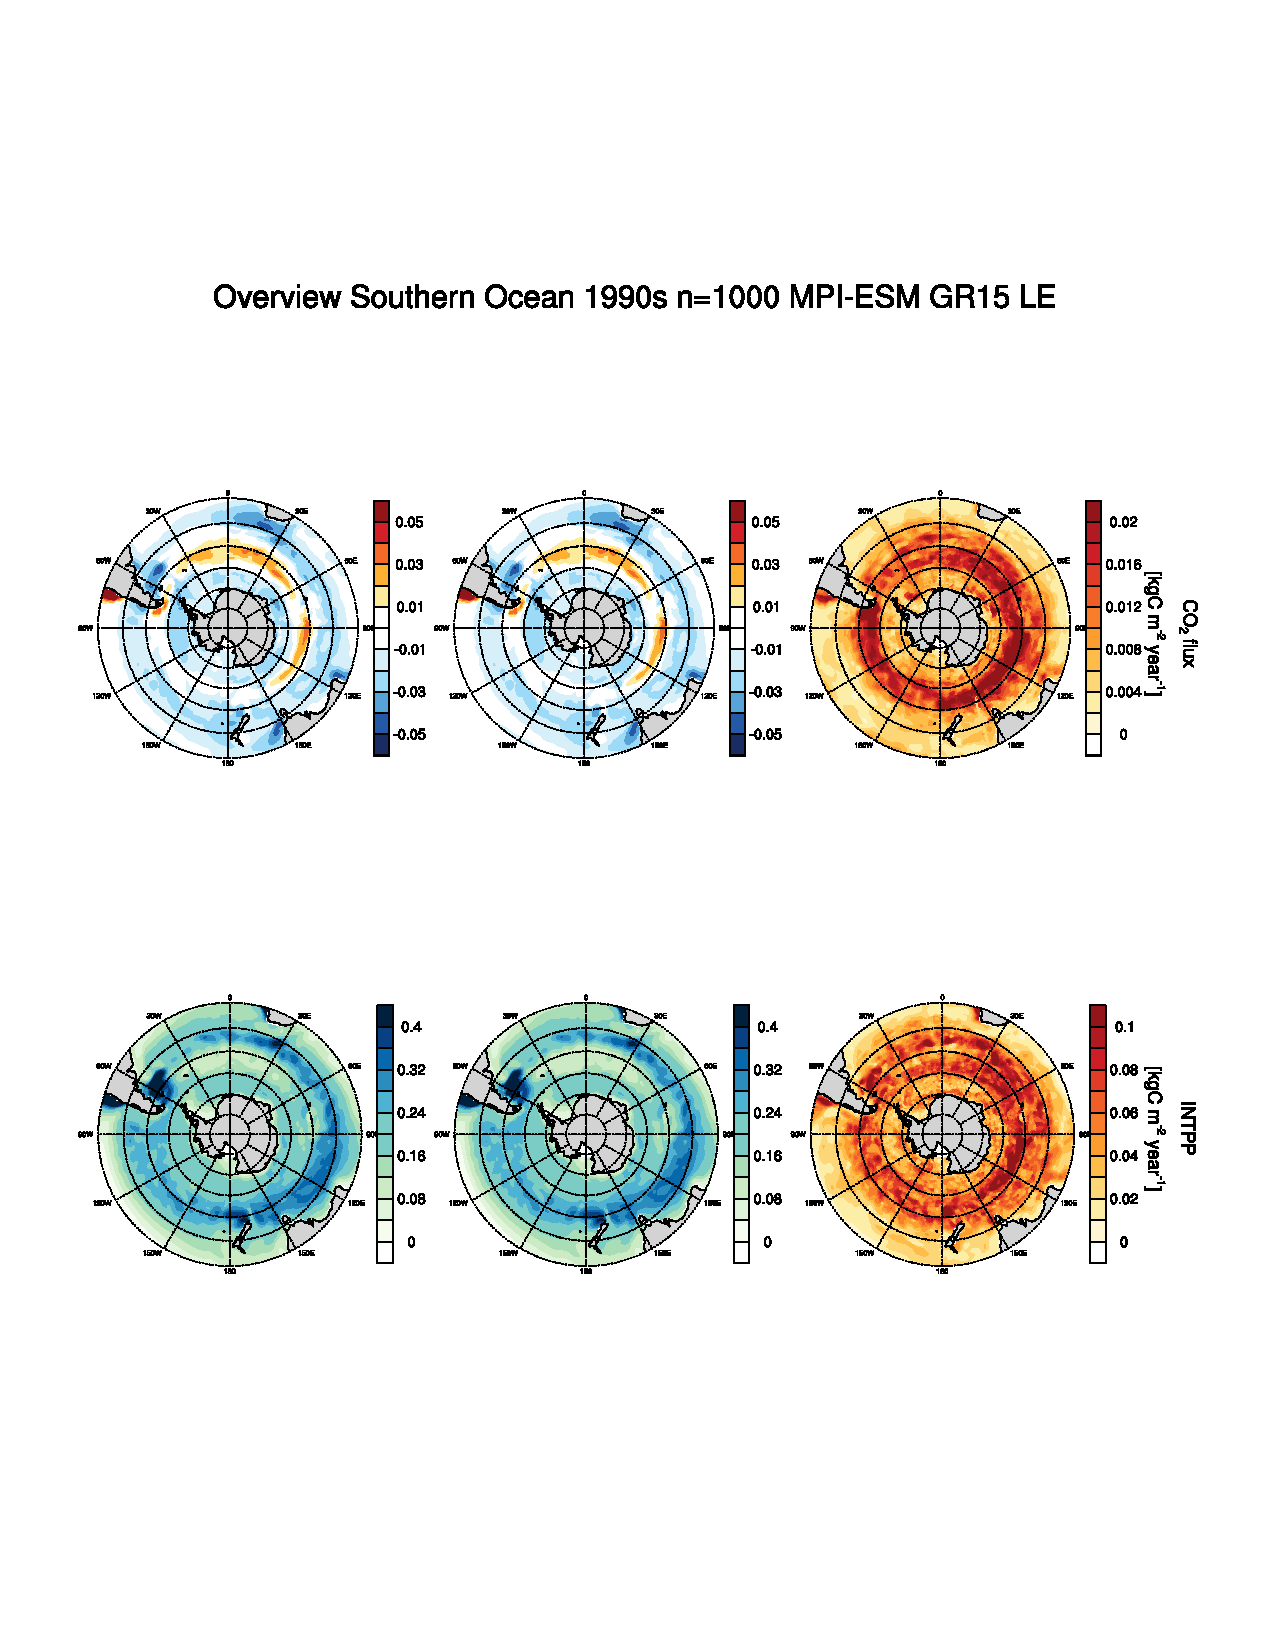
\includegraphics[scale=.45,trim=7.2cm 15cm 0cm 8cm,clip]{Overview_SO_co2flux_intpp_ens_t1990s.pdf} % from gfx folder
		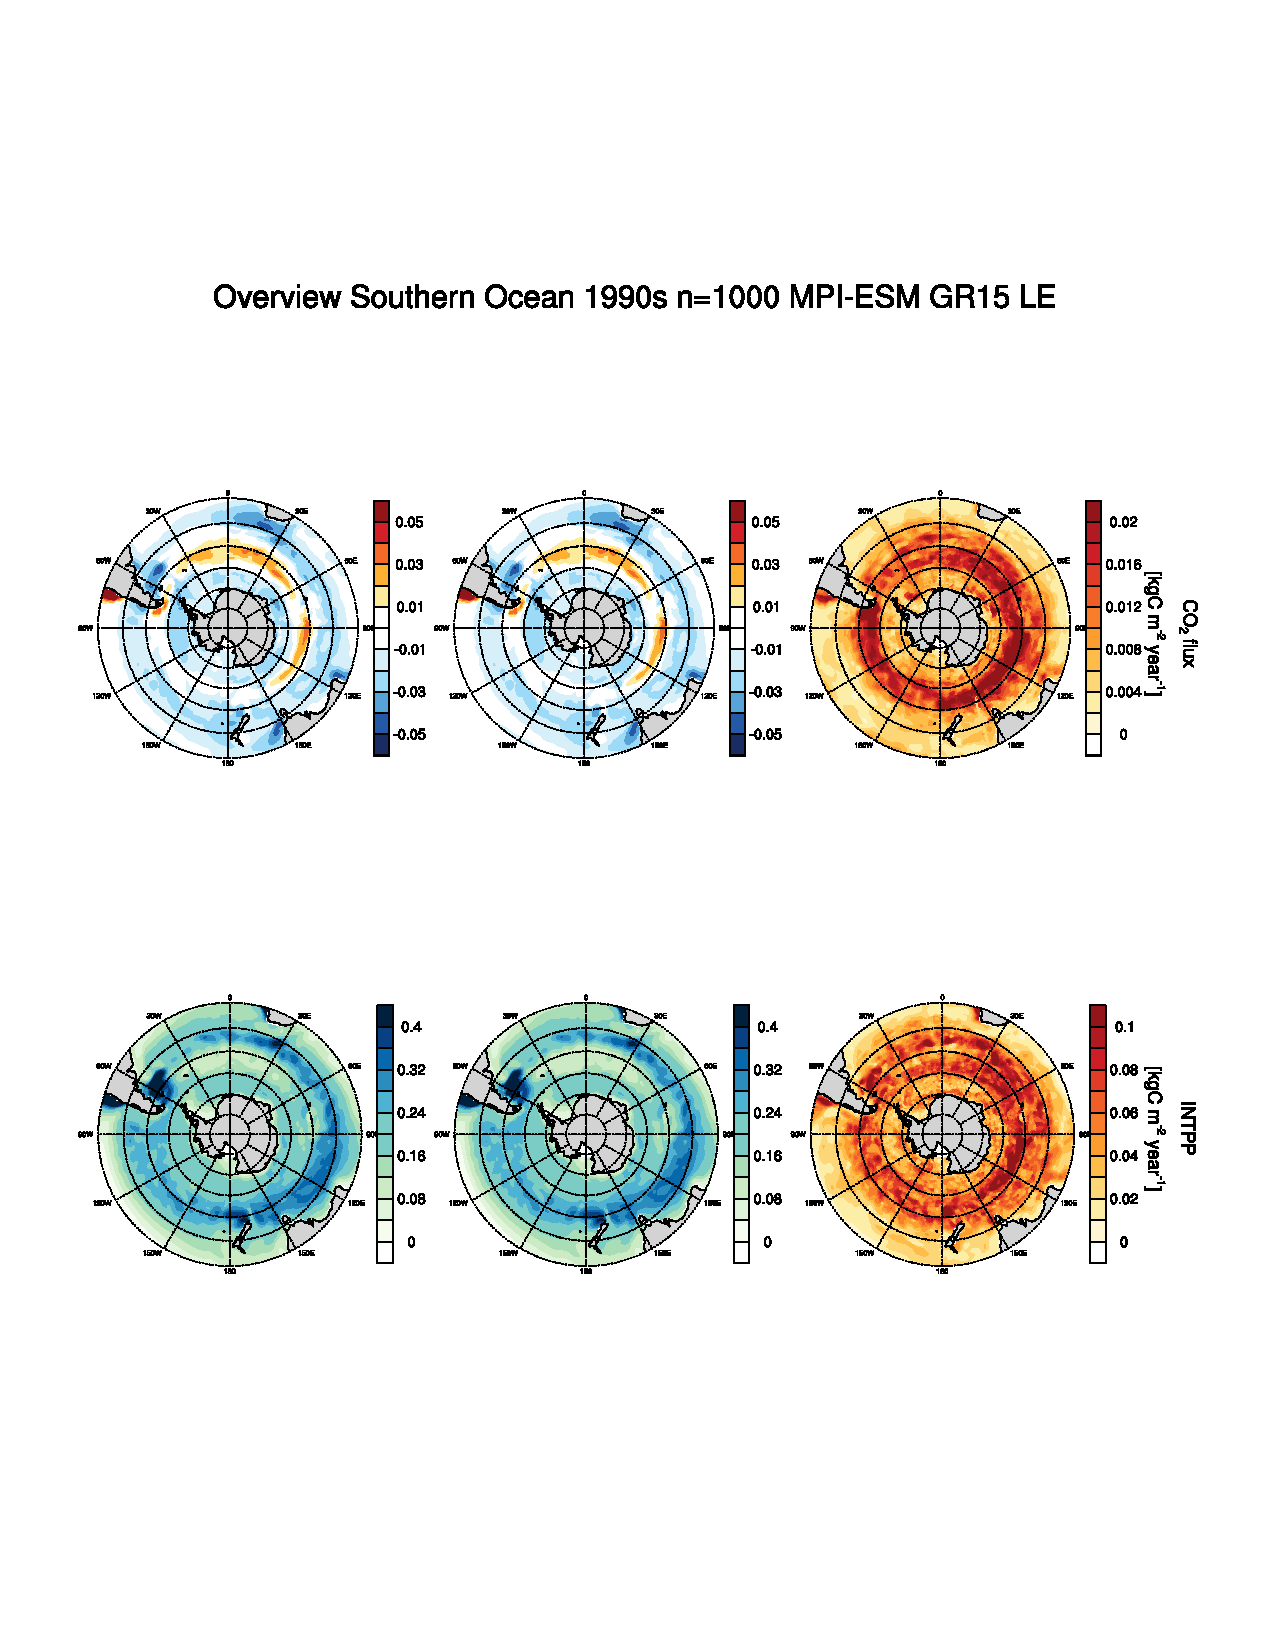
\includegraphics[scale=.45,trim=7.2cm 6.3cm 0cm 16cm,clip]{Overview_SO_co2flux_intpp_ens_t1990s.pdf} % from gfx folder
	\caption{Southern Ocean CO$_2$flux where negative values indicate ocean uptake (1$^{st}$) and primary production (2$^{nd}$): ensemble median (left) as forced signal and ensemble standard deviation (right) as internal variability \citep{Deser2012}}
		\label{fig:SOCS_ensmean_ensstd}
	\end{figure}
\end{frame}	
	
\begin{frame}{There are significant correlations of trends in CO$_2$flux,primary production and mixed-layer depth.}
	
	\begin{figure}
		\centering
		\includegraphics[scale=.8,trim=13.25cm 18.7cm 2.5cm 6cm,clip]{\member _positive_trend_8_obgc_overview_summer.pdf} %co2flux
\includegraphics[scale=.8,trim=13.25cm 15.9cm 2.5cm 9.2cm,clip]{\member _positive_trend_8_obgc_overview_summer.pdf} %intpp

\includegraphics[scale=.8,trim=13.25cm 13.1cm 2.5cm 12.1cm,clip]{\member _positive_trend_8_obgc_overview_summer.pdf} %nutlimf
\includegraphics[scale=.8,trim=13.25cm 7.3cm 2.5cm 17.8cm,clip]{\member _positive_trend_8_obgc_overview_summer.pdf} %zmld
\caption{Southern Ocean austral summer trends per per 8 years: CO$_2$flux (top left), vertically integrated primary production (top right), nutrient limitation (bottom right) and mixed layer depth (bottom left); hatched areas indicate where trends were below 5\% significance}
\label{fig:co2flux_intpp}
	\end{figure}
\end{frame}	

\begin{frame}{The decline in primary production at 50-60$^\circ$S is caused by reduced stability of the water column due to turbulent wind mixing\citep{Sverdrup1953}}

	\begin{figure}
		\centering
		\includegraphics[scale=.5,trim=10.5cm 13.2cm 0cm 7cm,clip]{\member _positive_trend_8_schwerpunkt_mixing_overview.pdf}
\caption{Trends in [m/8yrs] of average depth of vertical diffusivity due to wind (right); hatched areas indicate where trends were below 5\% significance}
\label{fig:wind_mixing}
	\end{figure}
	
\end{frame}

\begin{frame}{Water column stability is further decreased by cold upwelling water. This enhances the mixing power of the strengthening winds to pull phytoplankton deeper into the darker ocean.}
	\begin{figure}
		\centering
		\includegraphics[scale=.5,trim=1.2cm 13.2cm 11cm 7cm,clip]{\member _positive_trend_8_schwerpunkt_mixing_overview.pdf}
		\caption{Trends in [m/8yrs] for phytoplankton average depth; hatched areas indicate where trends were below 5\% significance}
	\label{fig:wind_mixing}	
	\end{figure}

\end{frame}

\begin{frame}{Deeper winter mixing delays primary production blooms in austral spring and lowers productivity all over the summer.}
	\begin{figure}[h]
		\centering
		\includegraphics[page=2,scale=.3,trim=0cm 6cm 0cm 5cm,clip]{\member _positive_trend_8_seasonality_intpp_zmld.pdf} % from gfx folder
		\caption{Seasonality of vertically integrated primary production (black) and mixed layer depth (red) at 50-60$^\circ$S over 8 years; thicker lines are later years}
		\label{fig:zmld_intpp_seasonality}
	\end{figure}
	
\end{frame}

\begin{frame}{Primary production decreases S30s because of nutrients, increases S40s because of temperature effect and stratification, decreases S50s because of instability.}
	
\end{frame}	
	
\begin{frame}{Anomalous outgassing trends in the Southern Ocean Carbon Sink can be explained by changes in primary production induced by changes in climate. We could not determine a ratio of summer primary production trend towards yearly upwelling trend.}
	
\end{frame}

\begin{frame}{Discussion on previous studies show different response of biology to increasing winds than other models which are in contrast to HAMOCC iron-limited.}
\citep{Lovenduski2008} \\
\citep{wang2012} \\
\citep{Hauck2013} \\

\end{frame}
	
	
\appendix

\begin{frame}[allowframebreaks]{References}
\baselineskip12pt
\bibliography{../Paper/SouthernOceanCarbonSink_new}

\bibliographystyle{abbrvnat}%unsrtnat}%abbrvnat}%plainnat}

\end{frame}	
	
	
	
\end{document}